\documentclass[a4paper]{article}


\usepackage{alphabeta} 
\usepackage{enumitem} 
\usepackage{mathtools}
\usepackage{amsmath, amssymb} 
\usepackage{amsthm}
\usepackage{cancel} 
\usepackage[margin=0.70in]{geometry} 
\geometry{left=3cm,right=3cm,top=2.4cm,bottom=2.4cm}	%the page geometry as defined, A4=210x297mm
\usepackage{graphicx}
\usepackage{wrapfig}
\usepackage{caption}
\usepackage{textcomp}
\usepackage{tabto}
\usepackage{layout}
\usepackage{bm}
\usepackage{minipage-marginpar}
\usepackage[dvipsnames]{xcolor}
\usepackage{hyperref}
\usepackage{dutchcal}
\usepackage{derivative}
\usepackage{esint}
%\usepackage{biblatex}
\usepackage{subcaption}
\usepackage{booktabs}\usepackage{derivative}
\usepackage[flushleft]{threeparttable}
\usepackage[capbesideposition=outside,capbesidesep=quad]{floatrow}
\usepackage{derivative}
\usepackage[thinc]{esdiff}
\usepackage{lipsum}
\usepackage{arydshln}
%%RENEW

\newtheorem{problem}{Άσκηση}
\newtheorem*{solution*}{Λύση}
\newtheorem{definition}{Ορισμός}[subsection]
\newtheorem{properties}{Ιδιότητες}[subsection]
\newtheorem{theorem}{Θεώρημα}[subsection]
\newtheorem{protash}{Πρόταση}[subsection]
\newtheorem{porisma}{Πόρισμα}[subsection]
\newtheorem{lemma}{Λήμμα}[subsection]
\newtheorem*{prooof}{Απόδειξη}
\newtheorem*{notes}{Παρατηρήσεις}
\newtheorem*{note}{Παρατήρηση}
\newtheorem*{app}{Εφαρμογή} 
\newtheorem*{example}{Παράδειγμα}
\newtheorem*{examples}{Παραδείγματα}


\newcommand\numberthis{\addtocounter{equation}{1}\tag{\theequation}}
%\renewcommand{\labelenumi}{\roman{enumi}}
\newcommand{\approxtext}[1]{\ensuremath{\stackrel{\text{#1}}{\approx}}}
\renewcommand{\figurename}{Εικόνα.}
\renewcommand{\tablename}{Πίνακας.}
%\renewcommand\refname{New References Header}
\renewcommand*\contentsname{Περιεχόμενα}
%\DeclareDerivative{\odv}{\mathrm{d}}


\begin{document}
\begin{titlepage}			%makes a title page. Remember to change the author, CID, username and group number to what is appropriate for you!
	\centering
	{\scshape\LARGE Εθνικό Μετσόβιο Πολυτεχνείο\par}
	{\scshape \LARGE Σ.Ε.Μ.Φ.Ε.\par}
	\vspace{1cm}
	{\huge\bfseries Ηλεκτροοπτικό Φαινόμενο, Προσδιορισμός Τάσης $V_{\lambda/4}$ Κρυστάλλου KDP \par}
	\vspace{1cm}
	{\Large\itshape Θωμόπουλος Σπύρος\par}		%remember to change these!
	
	%		{\large Group \@group\unskip\strut\par}
	{\large spyros.thomop@gmail.com/ ge19042@mail.ntua.gr\par \hfill \\}% 		%remember to change these!
	\vspace{1cm}
	{\large Ημερμονηνία Παράδοσης 05/04/2022\par}
\end{titlepage}

\subsection*{Σκοπός}


	Ο σκοπός της εν λόγω εργαστηριακής άσκησης είναι η μελέτη του ηλεκτροοπτικού φαινομένου Pockels για κρύσταλλο KDP και ο προσδιορισμός της τάσης $V_{\lambda/4}$, δηλαδή της τάσης η οποία αν εφαρμοστεί στον κρύσταλλο τότε αυτός θα δράσει ως πλακίδιο $\lambda/4$ προκαλλώντας διαφορά φάσης $\pi/2$ στις δύο πολώσεις μίας προσπίπτουσας δέσμης.
	
\subsection*{Θεωρία}


	Το ηλετρο-οπτικό φαινόμενο πρόκειται για το φαινόμενο κατά το οποίο μεταβάλλεται η διπλοθλαστικότητα ενός κρυστάλλου (διαφορετικοί δείκτες διάθλασης για κάθε πόλωση) κατά την εφαρμογή εξωτερικού ηλεκτρικού πεδίου. Ανεξάρτητα απ' το αν  η εν λόγω μεταβολή είναι μικρή ή μεγάλη, μπορεί να μεταφραστεί πάντοτε σε αρκούντως μεγάλη διαφορά φάσης αν το μήκος που διανύει η δέσμη εντός του κρυστάλλου είναι μεγαλύτερο από το μήκος κύματός της.

	Πιό συγκεκριμένα θα μελετηθεί το \textit{Διάμηκες Γραμμικό Ηλεκτροοπτικό φαινόμενο} (ή φαινόμενο Pockels) κατά το οποίο το εφαρμοζόμενο ηλεκτρικό πεδίο είναι παράλληλο με τον άξονα z του κρυστάλλου, κατά τον οποίο γίνεται και η διάδοση του κύματος. Θεωρούμε αρχικά ένα γραμμικά πολωμένο κύμα κατα 45$^o$ με: 
	\begin{align*}
		E_x = E_0 e^{i\omega(t - \frac{n_x}{c}z)} \\
		E_y = E_0 e^{i\omega(t + \frac{n_y}{c}z)}
	\end{align*}
	όπου έχουμε $n_x = n_0 - (n_0)^3r_{63}E_z/2$, $n_y = n_0 + (n_0)^3r_{63}E_z/2$, $r_{63}$ η ηλεκτροοπτική σταθερά του κρυστάλλου, $E_z$ το εφαρμοζόμενο πεδίο και θεωρούμε $z=L$ το μήκος του κρυστάλλου.
	
	Για να μετατρέψουν τον κρύσταλλό μας σε πλακίδιο $\lambda/4$, θα πρέπει να έχουμε διαφορά φάσης $\pi/2$: 
	\begin{align*}
		\Delta\phi = \phi_y-\phi_x = \left( (n_0)^3 r_{63}E_z \frac{\omega L}{c} \right) &\stackrel{V=LE_z,\omega/L=2\pi/\lambda}{=}	\left(\frac{2\pi V(n_0)^3r_{63}}{\lambda}\right) = \pi/2 \Rightarrow \\ 
		   &V_{\pi/2} = V_{\lambda/4} = \frac{\lambda}{4(n_0)^3r_{63}}
		\end{align*}
		
		Η πειραματική διάταξη φαίνεται στην Εικόνα 1. 
		\begin{figure}[h!]
			\centering
			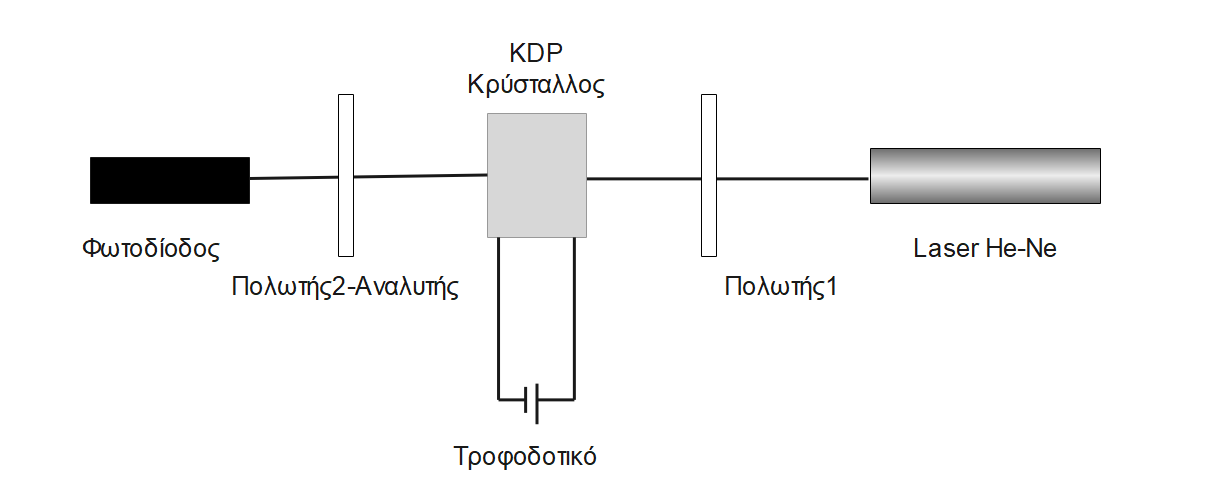
\includegraphics[scale=0.5]{pockels.png}
			\caption{ Πειραματική Διάταξη}
		\end{figure}
		
	Περιστρέφοντας τον Πολωτή 1 πετυχαίνουμε μία γωνία κατά την οποία το ΗΜ κύμα εξέρχεται από αυτόν με πόλωση $45^o$ προς τους άξονες x, y. Δεδομένου ότι έχουμε εφαρμόσει τάση $V_{\lambda/4}$ στον κρύσταλλο, το τελικό ΗΜ κύμα αφού εξέλθει από αυτόν θα είναι κυκλικά πολωμένο και συνεπώς περιστρέφοντας τον Πολωτή 2-Αναλυτή σε οποιαδήποτε γωνία θα έχουμε σταθερή ένδειξη στην μέτρηση από την φωτοδίοδο.
	
	Αν έχουμε απόκλιση των τιμών της τάσης στον κρύσταλλο και της γωνίας περιστροφής του Πολωτή 1 από τις απαιτούμενες για κυκλική πόλωση, τότε θα προκύπτει ελλειπτική 
\subsection*{Πειραματική Διαδικασία - Επεξεργασία Μετρήσεων}

	Αρχικα, αφού θέσουμε σε λειτουργία τα όργανα, μετράμε με την φωτοδίοδο την τάση που προκαλεί η ακτινοβολία υποβάθρου την οποία βρίσκουμε $V_{υποβ}=0.219V$. Τώρα εφαρμόζουμε στον κρύσταλλο μία αρχική τάση $V_{\lambda/4}=1.8kV $ ίση με την τιμή που περιμένουμε.
	
	Λόγω πειραματικών σφαλμάτων δεν περιμένουμε να βρούμε κυκλική πόλωση, αλλά ελλειπτική. Από αυτές, αυτή που είναι εγγύτερα σε κυκλική περιμένουμε να είναι σε γωνία του αρχικού πολωτή για την οποία η διαφορά μέγιστης-ελάχιστης ανιχνευόμενης ένταση γίνεται η μικρότερη δυνατή.
	
	Γι' αυτό, περιστρέφουμε τον Πολωτή 1 από $0-90^o$ με βήμα $10^o$ και για κάθε βήμα καταγράφουμε την μέγιστη και την ελάχιστη τάση καθώς περιστρέφουμε τον Αναλυτή. Αφού εντοπίσουμε την περιοχή με την ελάχιστη διαφορά των ακραίων τιμών τάσεων επαναλαμβάνουμε τα βήματα για αυτή την περιοχή γωνιών μέχρι να βρούμε αυτήν την γωνία που αντιστοιχεί στην ολική ελάχιστη διαφορά. 
	Τα αποτελέσματα φαίνονται στον Πίνακα 1.
	
	\begin{table}[h!]
		\centering
		\begin{tabular}{r|r|r|r}
		$\theta_{in}(\pm1^o)$ & $V_{min} (V)$ & $V_{max}$ (V)& $\Delta V = V_{max}-V_{min}(V)$\\ 
		\hline\hline
			0&0.310 &0.404 & 0.094\\
			10&0.262&0.405 & 0.143\\
			20&0.245&0.406 & 0.161\\
			30&0.296&0.404 & 0.108\\
			40&0.327&0.403 & 0.076\\
			50&0.344&0.403 & 0.059\\
			55&0.350&0.401 & 0.051\\
			\textbf{58}&\textbf{0.350}&\textbf{0.399} & \textbf{0.049}\\
			\textbf{60}&\textbf{0.351}&\textbf{0.399} & \textbf{0.048}\\
			62&0.349&0.401 & 0.052\\
			65&0.349&0.400 & 0.051\\
			70&0.348&0.403 & 0.055\\
			80&0.333&0.405 & 0.072\\
			90&0.306&0.406 & 0.100
		\end{tabular}		 
		\caption{(*)Παρατηρώ ότι στις 65$^o$ έχω μία πτώση της $\Delta V$ γεγονός που οφείλεται σε πειραματικά σφάλματα }
	\end{table}
	Οι μικρότερες διαφορές τάσης είναι για 58,60$^o$, άρα παίρνουμε $\theta_{\Delta\theta_{min}} = (59\pm1)^o$.
	Η γραφική παράσταση $\Delta V - \theta_{in}$  φαίνεται στην Εικόνα 2.
	\begin{figure}[h!]
		\centering
		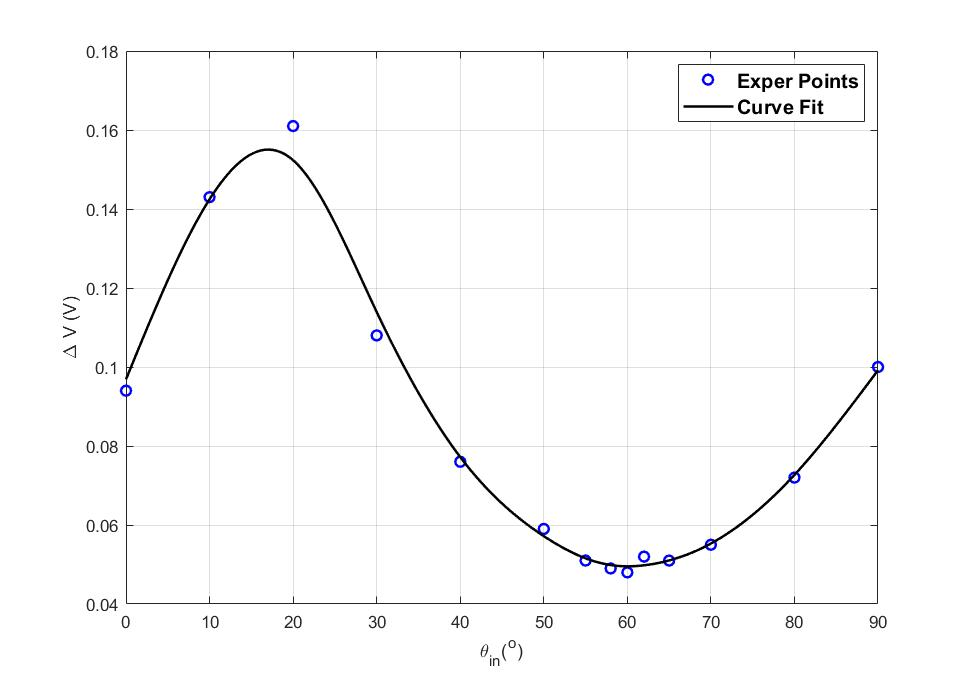
\includegraphics[scale=0.42]{plot1.jpg}
		\caption{Γραφική $\Delta V - \theta_{in}$}
	\end{figure}
	
	
	Το μέγιστο της διαφοράς των τάσεων που βλέπουμε για $20^o$ αντιστοιχεί σε κατάσταση η οποία είναι η πιό ''ελλειπτική'' από όλες τις υπόλοιπες, ενώ το ελάχιστο για $59^o$ είναι η σχεδόν κυκλική πόλωση που θέλουμε.
	
	Αφήνωντας τώρα την γωνία $\theta_{in} = 59^o$ μεταβάλλουμε την τάση που εφαρμόζουμε στον κρύσταλλο από $0.7-2.5kV$ προκειμένου να βρούμε αυτή που τον μετατρέπει σε πλακίδιο $\lambda/4$. Για κάθε τιμή της τάσης περιστρέφουμε τον αναλυτή και καταγράφουμε την μέγιστη και την ελάχιστη τάση, με σκοπό να βρούμε πάλι την διαφορά τους. Η μικρότερη από αυτές τις διαφορές αντιστοιχεί στην τάση $V_{\lambda/4}$. Οι μετρήσεις φαίνονται στον Πίνακα 2. 
	\begin{table}[h!]
		\centering
		\begin{tabular}{r|r|r|r}
		$V_{in}(kV)$ & $V_{min}(V)$ & $V_{max}(V)$ & $\Delta V(V)$ \\ 
		\hline\hline
		0.7&0.364&0.398&0.034\\
0.8&0.369&0.393&0.024\\
0.9&0.366&0.392&0.026\\
1.0&0.365&0.395&0.030\\
1.1&0.367&0.396&0.029\\
1.2&0.362&0.394&0.032\\
1.3&0.361&0.398&0.037\\
1.4&0.359&0.396&0.037\\
1.5&0.354&0.397&0.043\\
1.6&0.353&0.398&0.045\\
1.7&0.350&0.399&0.049\\
1.8&0.348&0.400&0.052\\
1.9&0.343&0.400&0.057\\
2.0&0.342&0.400&0.058\\
2.1&0.340&0.403&0.063\\
2.2&0.334&0.403&0.069\\
2.3&0.327&0.403&0.076\\
2.4&0.322&0.404&0.082\\
2.5&0.317&0.406&0.089
		\end{tabular}
		\caption{ }
	\end{table}
	Η γραφική παράσταση $V_{in} - \Delta V$ φαίνεται στην Εικόνα 3. 
	\begin{figure}[h!]
		\centering
		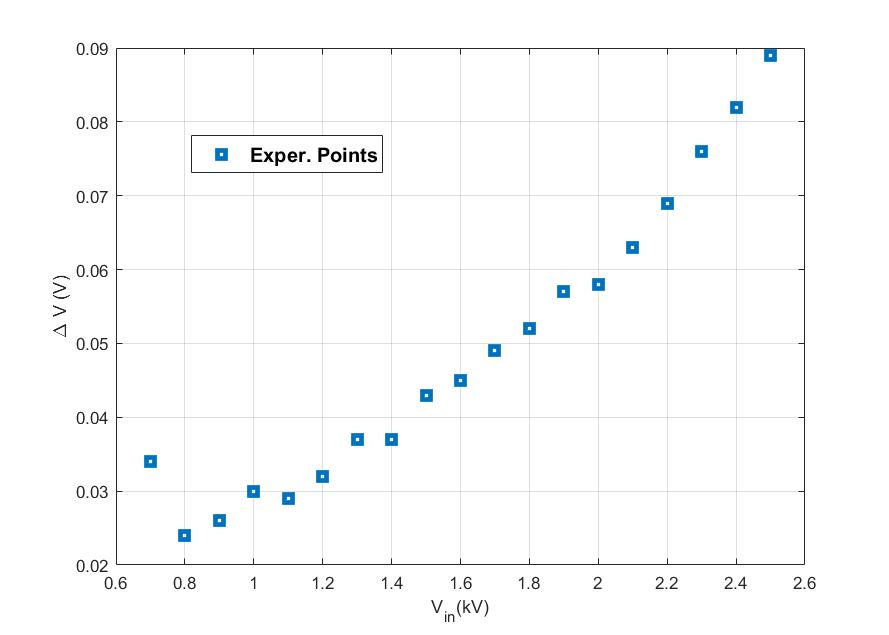
\includegraphics[scale=0.5]{plot2.jpg}
		\caption{$V_{in} - \Delta V$}
	\end{figure}
	
	Παρατηρούμε ότι η τάση $V_{\lambda/4}$ δεν είναι ίση με $1.8kV$ όπως περιμέναμε θεωρητικά, αλλά επιτυγχάνεται ελάχιστο για $V_{in} = 0.8kV$, τιμή πολύ μακρά από την αναμενόμενη. Τα σφάλματα που συνεισφέρουν στην εν λόγω απόκλιση οφείλονται σε σφάλματα ευθυγράμμισης της δέσμης laser, σε δικά μας σφάλματα κατά την πειραματική διαδικασία (π.χ. σφάλματα παράλλαξης), σε σφάλματα των οργάνων που οφείλονται στην πολυκαιρία (π.χ. η φωτοδίοδος μπορεί να μην ανταποκρίνεται αναλογικά στην προσπίπτουσα δέσμη) και τέλος στην φθορά του κρυστάλλου KDP επίσης από την πολυκαιρία.
\end{document}